%%%%%%%%%%%%%%%%%%%%%%%%%%%%%%%%%%%%%%%%%%%%%%%%%%%%%%%%%%%%%%%%%%%%%%%%
% Plantilla TFG/TFM
% Escuela Politécnica Superior de la Universidad de Alicante
% Realizado por: Jose Manuel Requena Plens
% Contacto: info@jmrplens.com / Telegram:@jmrplens
%%%%%%%%%%%%%%%%%%%%%%%%%%%%%%%%%%%%%%%%%%%%%%%%%%%%%%%%%%%%%%%%%%%%%%%%

\chapter{Desarrollo}
\label{desarrollo}

Como he comentado en el apartado de metodología \ref{metodologia}, el desarrollo del \gls{tfg} se divide en iteraciones, de las cuales ha habido un total de 9??\todo{añadir el total de iteraciones al final}, y en los siguientes apartados expondré cuál es el trabajo que se ha desarrollado en el transcurso de las mismas.
Por lo tanto, este apartado será el más extendido del \gls{tfg}, ya que en él explico detalladamente cuál es el trabajo que he ido haciendo, ordenado en el tiempo, y dividido en los tempos que me he reunido con mi tutor.

\section{Primera iteración: desarrollo del motor}
El \textbf{7 de julio de 2020} nos citamos por la herramienta Google Meet, y hablamos sobre cuál era mi objetivo con este \gls{tfg}, lo definimos y presentamos la propuesta. Además, como no tenía conocimientos sobre motores de videojuegos, me sugirió empezar viendo su curso para desarrollar un motor en C/C++. No concertamos una segunda cita ya que empezaba la época de verano, y quedamos en que cuando comenzara el curso y hubiera desarrollado mi motor volvería a ponerme en contacto con él.

\subsection{Script de construcción del proyecto}
Lo primero que hice fue, antes de ponerme a programar el motor, crear el archivo Makefile, este es el fichero que la herramienta Make ya mencionada en la página \pageref{herramientas} utiliza como Build Script. De esta forma no tendría que compilar todos los archivos uno a uno. Y además, separando las librerías del resto del código, así no tendrían que ser re-compiladas cada vez que necesite crear un ejecutable, ya que este es un proceso que tarda unos segundos pero se repite muchas veces, por lo que estos segundos ahorrados a lo largo del desarrollo podrían llegar a ser muchos minutos, incluso horas, de espera ahorrados.

Como no voy a explicar todo el archivo línea por línea, lo haré con las partes más importantes del mismo. 
\begin{itemize}
	\item La macro \textbf{COMPILE}, recibe cinco parámetros. Es usada para compilar todos los objetos antes de ser enlazados. Recibe los siguientes parámetros:
	\begin{enumerate}
		\item Compilador a usar (gcc, g++, clang++, etc.)
		\item Nombre del objeto que se genera
		\item Archivos de código fuente
		\item Dependencias
		\item Flags para el compilador
	\end{enumerate}
	\begin{lstlisting}[style=C, caption={Macro Compile del Makefile},label=C_code]
		define COMPILE
		$(2) : $(3) $(4)
			$(1) -c -o $(2) $(3) $(5)
		endef
	\end{lstlisting}
	\item La instrucción \textbf{\$(APP)} o \textbf{game}, que es el nombre del ejecutable final. 
	\begin{itemize} 
		\item Depende de todos los objetos. 
		\item Enlaza todos los objetos y librerías, y genera el ejecutable
	\end{itemize}
	\begin{lstlisting}[style=C, caption={Enlazado de los objetos y las librerísa para generar el ejecutable.},label=C_code]
	$(APP) : $(OBJSUBDIRS) $(ALLOBJ)
		$(CC) -o $(APP) $(ALLOBJ) $(LIB) $(CCFLAGS)
	\end{lstlisting}
	\item La instrucción \textbf{clean}, que elimina los objetos para re-compilarlos desde cero.
	\item La instrucción \textbf{libs} y \textbf{libs-clean}, que compila y elimina pero con las librerías.
\end{itemize}
Dentro de la carpeta lib tenemos otro Makefile que sirve para compilar las librerias, las cuales tienen su propio Makefile también, muy parecido al ya mencionado.

\subsection{Motor de videojuego}
Comenzamos el desarrollo del videojuego creando el motor, pues sin él, no se puede avanzar con los otros puntos. Se trata de un motor \gls{ecs}\footnote{Conocido en español como Sistema de Entidades y Componentes. Es un patrón de desarrollo para motores de videojuegos.} el cual se basa en que las entidades son manejadas por el motor, mientras que los componentes (como físicas, renderizado, colisiones, etc.) son añadidos desde el juego. Pero el motor es el que se encarga de añadir los componentes a las entidades o destruirlos. Y los sistemas son los encargados de actualizar el estado de los componentes.

Para que el motor se comporte de manera eficiente con la caché, todos los componentes de un mismo tipo se almacenan seguidos en memoria, para que así, cada sistema del juego pida un solo tipo de componente de todas las entidades del juego. Ya que se ha demostrado que leer un dato de la caché es, de media, 200 veces más rápido que leerlo de la RAM, y cuando el programa pide un dato, no solo se carga ese dato pedido, sino un stream de datos. Como se puede apreciar en la figura \ref{Memoria RAM y CPU}.
\begin{figure}[h]
	\centering
	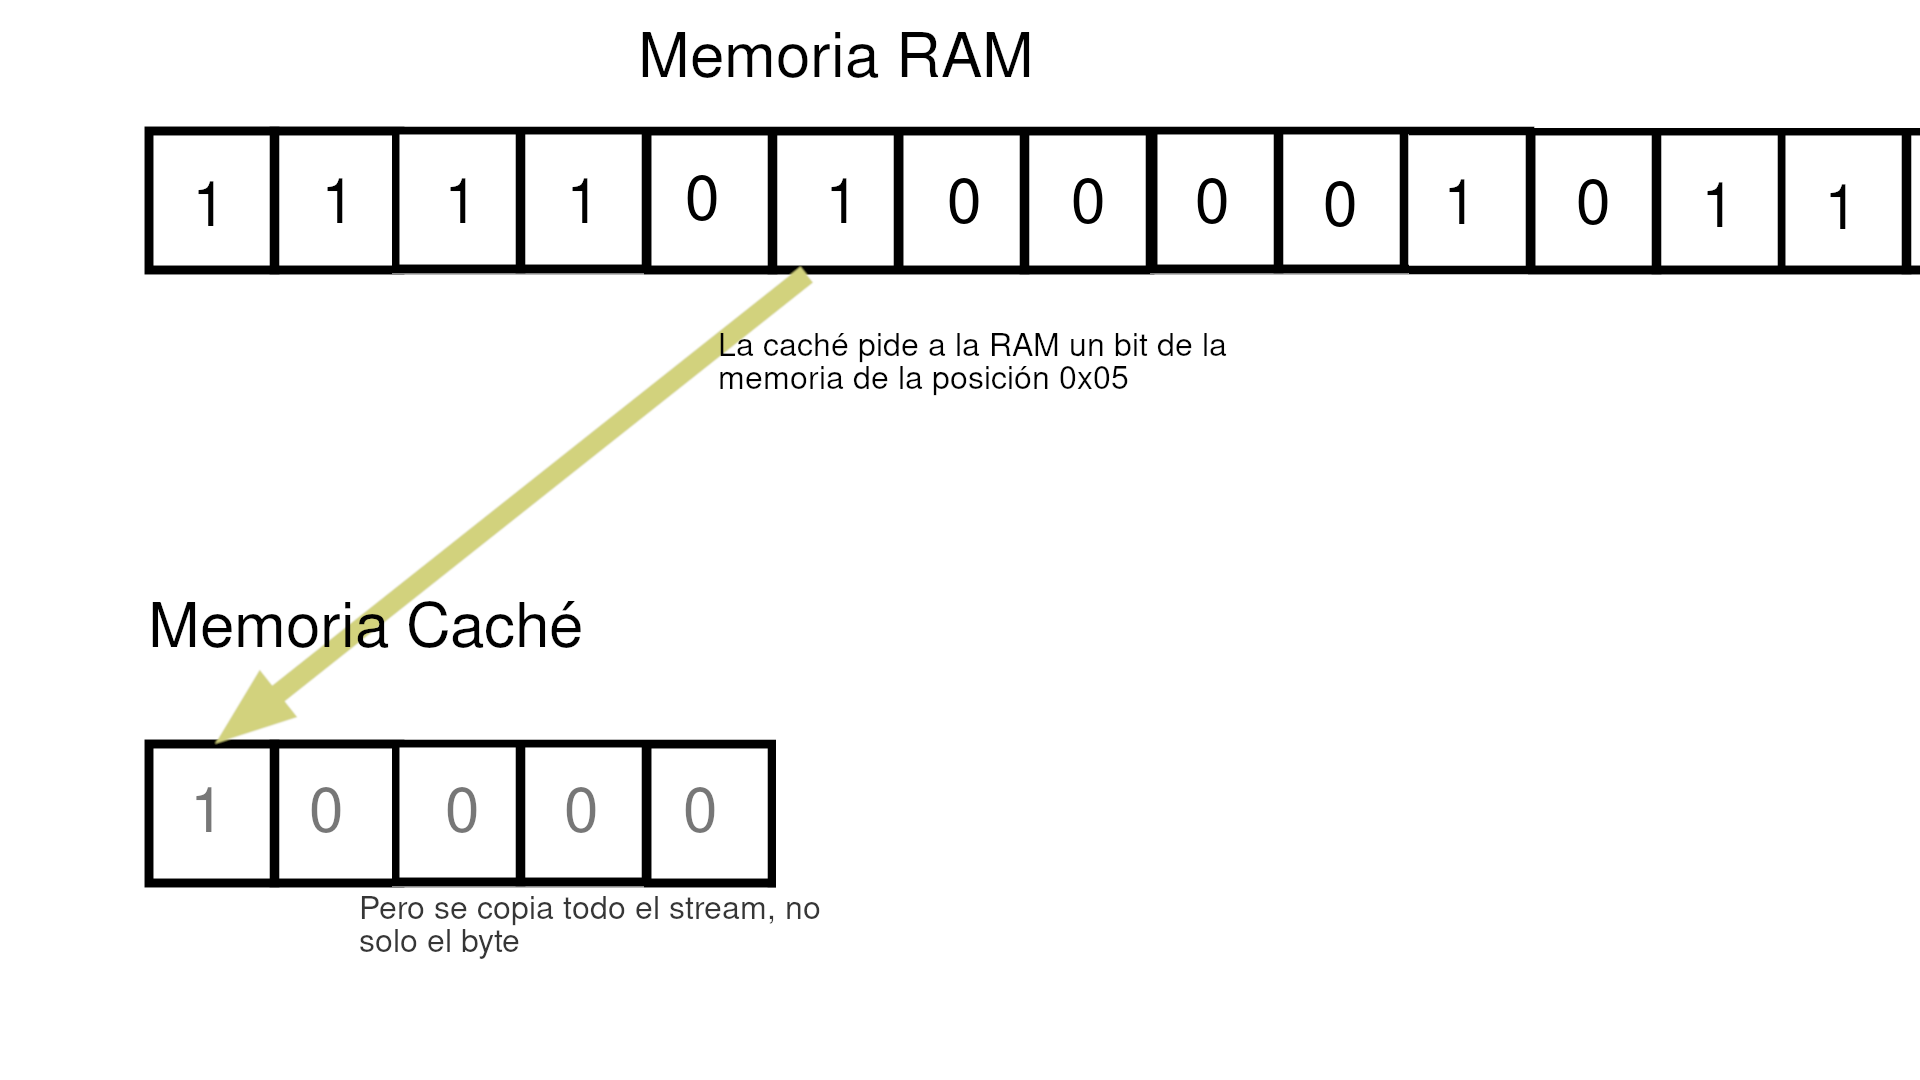
\includegraphics[width=15cm]{archivos/imagenes/comportamiento-memoria-cpu-ram.png}
	\caption{Comportamiento de la memoria CPU cuando lee de la RAM.}
	\label{Memoria RAM y CPU}
\end{figure}

¿Cómo se pueden alinear los datos en memoria según su tipo? La implementación ha sido usando la librería unordered\_map de C++, con la cual podremos usar un mapa, es decir, una estructura de datos en la que uno es el identificador (el tipo de dato, en este caso), y otro es el valor almacenado (un vector de componentes, en este caso).  Esto trae un problema consigo, porque el ``tipo de dato'' no es un tipo básico en C++, esto explicaré más adelante cómo lo solucionaremos. 

Cada sistema es encargado de un tipo de componente, para así poder recorrer la memoria de forma lineal como ya hemos mencionado antes (el sistema de físicas recorre todos los componentes de físicas existentes en el motor), y así optimizar el uso de la caché. Aunque como veremos adelante, eso no es del todo sencillo, porque en ocasiones, actualizar el estado de un componente depende del estado de un segundo\footnote{Un ejemplo de esto es al actualizar los componentes de colisiones, es inevitable tener que solicitar el componente de física.}.
\\
Todas las clases del motor están dentro del espacio de nombres \textbf{ECS}.

\begin{figure}[h]
	\centering
	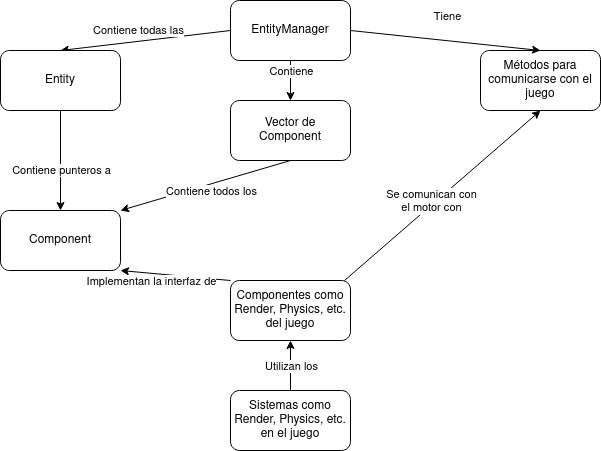
\includegraphics[width=15cm]{archivos/imagenes/Diagrama-funcionamiento-motor.png}
	\caption{Para qué se utiliza EntityManager.}
\end{figure}

Como vemos en la anterior imagen, la clase EntityManager\_t es la clase que usará el juego para comunicarse con el motor. Tiene los métodos necesarios para almacenar, solicitar y borrar tanto entidades como un componente de una entidad. Estos componentes son almacenados en m\_components, así que EntityManager\_t tiene un fuerte acoplamiento con ComponentStorage\_t, y si quisiéramos otra implementación del motor donde los componentes no sean parte de las entidades, haría falta aplicar cambios sobre este acoplamiento.

La clase Entity\_t tiene un vector de punteros hacia sus componentes, la ventaja de esto es que no hace falta que el componente tenga un ID, y por lo tanto, la búsqueda del componente es más rápida. El inconveniente es que hay que tener mucho cuidado con dónde está almacenado el componente, ya que el encargado de darle una zona en la memoria es ComponentStorage\_t, y si este modifica la posición del componente, el puntero en Entity\_t no apuntará a la zona correcta de la memoria. 

Por último, el motor también proporciona una interfaz para la comunicación entre la entrada de teclas en el juego y el sistema operativo. Esto lo hace utilizando algunas funciones de la librería TinyPTC, que se activan cuando una tecla es pulsada.\footnote{Para un desarrollo más amplio de cómo funcionan estas funciones, ver el curso de \citep{CursoMotorC++}.}

\subsection{Dificultades a destacar}
Algunas de las dificultades de crear un motor genérico, que pueda aceptar cualquier tipo de componente es que hay que hacer las funciones template, de no ser así, cada vez que queramos añadir un nuevo componente habría que añadir una nueva función, la cual sería una copia de otra y eso podría generar errores futuros al tener que cambiar lo mismo en todas las copias. Y no solo eso, el mayor problema sería que el motor no estaría desacoplado del juego, y no sería útil para cualquier juego, sino habría que modificarlo en función del juego que queramos crear.

Un segundo problema es que la clase Entity\_t almacena punteros a Component\_t, pero como ComponentBase\_t hereda de Component\_t es posible que trabaje con los componentes del juego. ¿Por qué añadir este nivel de indirección? El problema lo hemos mencionado antes: el tipo de un componente no es un tipo básico de C++. Por lo tanto, no podremos usar una estructura de mapa para almacenar los componentes del juego según el tipo de forma lineal en memoria.
\\
Lo solucionamos de la siguiente manera: la clase Entity\_t almacena un unordered\_map de ``tipo de componente'' a ``puntero a Component\_t''. Component\_t tiene un método estático getComponentTypeID() que devuelve un entero que será el identificador único del componente durante la ejecución del programa. De esta manera, el juego podrá añadir tantos tipos de componente distintos como quiera, sin tener que preocuparse por el identificador, que es tarea del motor.
\begin{lstlisting}[style=C-color, caption={Cómo poder tener un número variable de componentes, sin tener que añadir un nuevo identificador con cada componente nuevo.},label=C_code-color]
	static ComponentTypeID_t getComponentTypeID() noexcept {
		static ComponentTypeID_t typeID { ++nextTypeID };
		return typeID;
	}
\end{lstlisting}
Pero, ¿qué significa el anterior código? Para entenderlo, hemos de saber para qué sirve la palabra reservada ``static'': cualquier variable que sea estática existirá al principio del programa, y continuará hasta el final de la ejecución del mismo. Por lo tanto, el método getComponentTypeID() devolverá siempre el mismo identificador, ya que typeID se define una sola vez en la ejecución del programa, y no cada vez que se llama al método, y nextTypeID es un miembro estático de la clase padre Component\_t que inicialmente es cero.
\\
Pero esto ocasiona el problema de que todos los componentes devolverán el mismo identificador. ¿Cómo hacemos que cada componente tenga el suyo propio? C++ tiene templates, lo que significa que, en tiempo de compilación, un código template se replicará por cada tipo diferente que haya sido instanciado la clase template. Por lo tanto, cada componente del juego, deberá heredar de ComponentBase\_t, de esta manera se crearán tantos ComponentBase\_t con su método estático getComponentTypeID() como componentes distintos tenga el juego.

Otro problema relacionado con la creación de un motor genérico es que, en algunos casos, las funciones del juego se usarán en un ámbito constante, y otras no, por lo que las funciones que queramos que sirvan para ambos casos, han de estar replicadas de forma que devuelvan un valor constante o no. El problema del código repetido que se solventa haciendo uso del las conversiones con static\_cast<>(), podemos ver un ejemplo a continuación:
\begin{lstlisting}[style=C-color, caption={Ejemplo de conversion de un método constante a no constante},label=C_code-color]
	template<typename CMP_t>
	const CMP_t* getComponent() const {
		auto type = CMP_t::getComponentTypeID();
		auto it = m_components.find(type);
		if(it != m_components.end()) 
		return static_cast<CMP_t*>(it->second);
		return nullptr;
	}
	
	template<typename CMP_t>
	CMP_t* getComponent() {
		const CMP_t* cmp = const_cast<const Entity_t*>(this)->getComponent<CMP_t>();
		return const_cast<CMP_t*>(cmp);
	}
\end{lstlisting}
Hay que recordar siempre, que las conversiones han de ser de un método constante a uno no constante. De no ser así, podría suceder que el método no constante modifique algo, y devolvamos algo que ha mutado en el método constante.

\section{Segunda iteración: desarrollo del Pong}
El \textbf{29 de octubre de 2020} tuvimos la segunda iteración donde le conté a mi tutor lo que había aprendido y acordamos los siguientes objetivos:
\begin{itemize}
  \item Aprender a usar \LaTeX.
  \item Comenzar la estructura de la memoria.
  \item Ver el curso de Yaser Abu-Mostafa sobre \gls{ml}.
  \item Crear un pong donde las palas se controlen aplicando aceleración y no velocidad.
  \item Almacenar los datos de la partida en \gls{csv}.
  \item Programar un perceptrón.
\end{itemize}

\subsection{Creación del juego}
Al igual que, para continuar con el desarrollo del TFG, lo primero era crear un motor funcional, antes de poder implementar los conocimientos de \gls{ia} hay que crear un juego. Como mencioné en la introducción (página \pageref{introduccion}), esta es la parte más creativa, y puede que sea la parte que más tiempo me lleve pero no necesita prácticamente mucha formación. Por lo que, lo primero que voy a hacer es programar el clásico juego del Pong para que, posteriormente, la pala rival sea controlada por un perceptrón. 
\\
El juego tiene una estética simple, hecha sin sprites, solo coloreando en la ventana un color uniforme para cada entidad:
\begin{figure}[h]
	\centering
	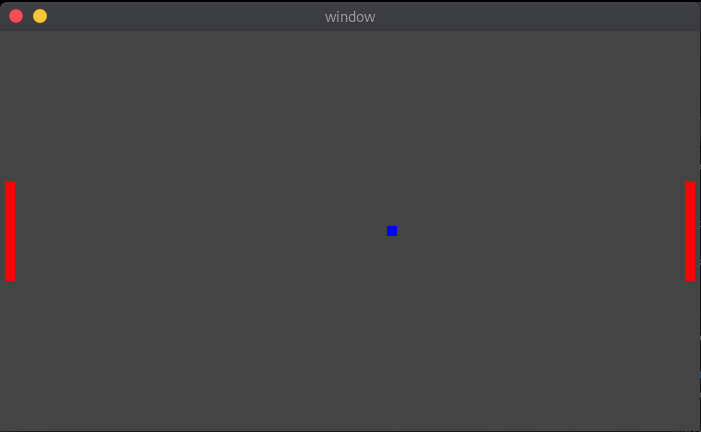
\includegraphics[width=15cm]{archivos/imagenes/pong.png}
	\caption{Imagen del primer juego, Pong.}
\end{figure}

Además, al juego le he añadido un menú, en el que eliges si quieres jugar contra un humano, para recoger los movimientos de la pala, si quieres entrenar la \gls{ia}, con algún \gls{csv} de datos de alguna partida anteriormente jugada, y una tercera opción de jugar contra una \gls{ia}. Y por supuesto la opción de salir.
\begin{figure}[h]
	\centering
	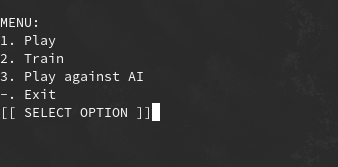
\includegraphics[width=15cm]{archivos/imagenes/menu-del-pong.png}
	\caption{Primer menú del juego.}
\end{figure}

Programar el juego no fue algo especialmente complicado, dado que durante el curso de motor de videojuegos en C++ de \citefullauthor{CursoMotorC++}, se implementan sistemas y componentes como los de colisiones, físicas, etcétera, muchos solo había que adaptarlos al Pong y ya funcionaban. Además tuve que añadir algunos extra como un sistema de puntuación, por ejemplo. Y no tuve que hacer nada de arte gráfico por el momento, ya que con unos rectángulos que se pueden generar con un for, era suficiente para entender el juego, como se puede ver en la imagen del juego.

\subsection{Resolución del resto de trabajo}
Almacenar los datos en un \gls{csv} no fue una tarea extremadamente difícil. Cada sistema tiene un método dump() y un array donde se almacenan los datos de cada frame, y cada 100 frames se guarda en un \gls{csv} los datos de ese sistema durante la partida.

La estructura de la memoria la estoy haciendo en base la plantilla que nos proporciona José Manuel Requena en GitHub \footnote{\url{https://github.com/jmrplens/TFG-TFM\_EPS}}, y fijándome en la estructura del libro de Yaser y los \gls{tfg} de mis compañeros anteriormente mencionados.

Y por último, he comenzado a intentar implementar, sin éxito, los conocimientos sobre el perceptrón. La pala rival no responde en función de los parámetros del juego después de haber sido entrenada, por lo que estoy entendiendo mal los conceptos de \gls{ml} explicados en \citep{LearningFromData}. En la próxima cita con mi tutor le expondré este problema para ver cómo podremos darle solución.

\section{Tercera iteración: problemas con el aprendizaje}
El \textbf{26 de noviembre de 2020} volvimos a quedar para ver mi trabajo durante el último mes, y nos encontramos con varios problemas. Los problemas serían los objetivos para la próxima iteración, y fueron los siguientes.

\begin{enumerate}
	\item A pesar de tener formación en inglés y de haber cursado alguna asignatura en la carrera sobre \gls{ia}, me resultaba difícil comprender los conceptos que Yaser explicaba en el curso, así que mi tutor, me recomendó la lectura del libro en el que se basan estas charlas, en el cual se extiende más y hace más fácil la comprensión del mismo.
	\item A pesar de tener el juego del Pong ya funcionando, el día de antes estuve añadiendo código, cosa que hizo que dejara de funcionar. El código estaba bajo el control de versiones de Git, sin embargo, no sabía utilizar la herramienta por completo así que no supe volver a una versión anterior.
	\item No sabía cómo comenzar a escribir mi \gls{tfg} ni qué escribir en cada una de sus secciones.
\end{enumerate}

Después de estos problemas, ralentizamos el ritmo de desarrollo y acordamos que para la siguiente iteración: habría aprendido a usar Git por completo, habría revisado algunos de los \gls{tfg} de mis compañeros, con un posterior desarrollo del mío propio, y habría leído \textit{Learning from data: a short course} \cite{LearningFromData}

Durante esta iteración no hubo un gran avance del proyecto, debido a que todas las tareas que propusimos fue que arreglara los errores que había tenido hasta el momento, y el tiempo entre esta y la siguiente era más reducido de lo normal.

\section{Cuarta iteración: juego con el perceptrón}
El \textbf{17 de diciembre de 2020} tuvimos la última cita del año, revisamos los objetivos marcados en la anterior iteración y ya había desarrollado brevemente cada campo de la memoria del \gls{tfg}, implementado el perceptrón y aprendido a usar Git. Sin embargo, no habiendo terminado de leer \textit{Learning from data: a short course}, y con las ideas un poco confusas, el perceptrón no respondía correctamente, por lo que los objetivos para la siguiente iteración serían:
\begin{itemize}
  \item Completar toda la memoria con las cosas hechas hasta el momento.
  \item Ver las clases de Razonamiento Automático de mi tutor.
  \item Arreglar la implementación del perceptrón.
  \item Hacer funcionar el perceptrón dentro del juego.
  \item Rehacer el sistema de recogida de datos en \gls{csv}.
\end{itemize}

\subsection{Desarrollo total del perceptrón}
El problema principal con el perceptrón fue que, debido a algunas similitudes entre entrenar y jugar, implementé el código de tal forma que todo estaba en la misma clase. Mi tutor me explicó que la parte del entrenamiento está separada del juego y me dijo que viese las clases de Razonamiento Automático, de esta manera conseguiría aclarar las ideas tan dispersas que tenía.

Lo que hace el perceptrón es recibir los datos relevantes de la partida, como son las físicas de la pelota y del jugador controlado por la \gls{ia}. Entonces, los datos son una X de la siguiente fórmula, y los pesos del perceptrón ya entrenado son representados con una W.
\begin{equation}
	\sum_{i=0}^nX_{i}*W_{i}
\end{equation}
El resultado de ese sumatorio será positivo o negativo, y no es necesario añadir en la fórmula el límite, sino que el límite es 0 ya que entre los datos se ha añadido el threshold como una entrada con valor 1, y entre los pesos se ha añadido uno extra al principio para que se ajuste al igual que el resto de pesos. En el caso de dar positivo, significará que la suma ha superado el threshold, lo que significa que la \gls{ia} manda al juego pulsar esa tecla de la pala, y en caso de ser negativo no. A cada tecla (arriba y abajo) le corresponde un perceptrón, que es el que decide si esta es pulsada o no.

Para entrenar al perceptrón, paso previo para jugar contra él porque sino, no existirá un fichero con la configuración del mismo, lo que hago es:
\begin{enumerate}
	\item Generar un array de pesos aleatorios y calcular el error que generan estos pesos.
	\item Se repite N veces el siguiente proceso:
	\begin{enumerate}
		\item Se calcula el error de los pesos que se quiere ajustar.
		\item Si este perceptrón con estos pesos es mejor que el mejor hasta el momento (tiene un error menor), se guarda.
		\item Del perceptrón ajustado, se elige uno al azar entre todos los puntos que no ha acertado si pulsar o no pulsar. 
		\item Si la tecla no fue pulsada, y debía serlo, se suma al peso el valor del input del perceptrón. Si la tecla fue pulsada, y no debía serlo, se resta. (Es decir, teniendo M entradas, la operación de suma o resta se hace desde 0 hasta M, al peso i se le suma/resta el input i).
	\end{enumerate}
	\item El perceptrón que haya dado menor error se guarda en un fichero para poder ser usado en el juego.
\end{enumerate}

El perceptrón ya funcionaba correctamente después de ver las primeras clases de Razonamiento Automático, ya que conseguí entender las dudas que me quedaban sobre el tema. Dando un resultado totalmente jugable, ya que no era invencible, ni tampoco tan malo como para no convertirse en un reto. El error que no permitía funcionar de forma correcta era el sobreentrenamiento. El \gls{csv} de datos tenía una cantidad mucho mayor de ejemplos de ``no pulsar'', y muy pocos de ``sí pulsar'', por lo que en la mayoría de casos, el perceptrón entrenado se quedaba parado. Esto tenía varias posibles soluciones, entre ellas ajustar el cálculo del error (es decir, que un fallo de no pulsar cuando sí hay que hacerlo subiese más el valor error), y por la que opté yo, que era ajustar los datos de tal manera que quedasen distribuidos la mitad del ejemplo de frames pulsando y la otra mitad no pulsando. Esto trajo otro pequeño inconveniente, y era que los datos extraídos de ``no pulsar'' eran del principio de la partida, y esos frames de ejemplo no eran lo suficientemente representativos, por lo que opté por coger los frames aleatorios.

\subsection{Desarrollo de una red neuronal}
Además, en las clases de Razonamiento Automático, mi tutor explica cómo funciona una red neuronal y cómo programarla, incluso, invita a los alumnos a crearla de tal forma que sea diferente a la ya creada por él, sin el uso de la librería vector de C++ para conseguir una mayor eficiencia en lo que se refiere a los tiempos de ejecución. Por lo que después de aprender los conceptos con sus clases, me dispuse a programar mi propia red neuronal para después introducirla en el juego cuando este se convirtiera en algo más complejo que una pala rebotando una bola, sin embargo, no era consciente de las facilidades que aporta la clase vector, y me topé con varios problemas durante el desarrollo.
\\
Algunos de estos problemas fueron, tener que sobrescribir el constructor de copia por no comportarse cómo deseaba, tener que manejar el puntero de los datos según si se quería contar el threshold o no (recordemos que uno de los motivos por los que haría una implementación propia de la clase vector sería para obtener más eficiencia a la hora de leer los datos), etc.
\\
El hecho de tener que detenerme a estudiar cómo funcionan algunas de las facilidades que aporta vector, y escribir las partes de la memoria que faltaban me llevó todo el tiempo que quedaba hasta esta quinta iteración. Ya había solventado los problemas de la anterior y había alcanzado los objetivos propuestos, por lo que llegué con todo el trabajo hecho a esta.

\subsection{Recogida de datos de la partida}
Además, un segundo problema de concepto fue el cómo recoger los datos. En primera instancia cada sistema se encargaba de recoger sus datos en el \gls{csv}, de tal manera que como los sistemas necesarios para que la \gls{ia} aprenda son las físicas y el sistema de input, había dos archivos que correspondían a la misma partida, con distinto nombre y distintos datos, pero tremendamente acoplados, por lo que mi tutor sugirió que los recoja de manera externa a sus sistemas, todos los datos necesarios en un mismo \gls{csv}, así que ese era otro objetivo para la siguiente iteración. 

Y por último, me dijo que no era necesario almacenar datos en array, ya que el juego no es tan complejo como para que se ralentice por abrir y escribir un archivo en cada frame. Conseguí solucionarlo rápidamente. Al principio de la partida creo unas referencias a los objetos que necesito guardar, y en cada frame abro el archivo y lo escribo con los datos actuales. No es la forma más eficiente de hacerlo, pero para un juego tan sencillo funciona perfectamente.

\section{Quinta iteración: mejorando el juego}
El \textbf{14 de enero de 2020} tuvimos la siguiente iteración, los objetivos marcados para la siguiente iteración han sido más ambiciosos de lo normal, así que no es necesario que estén completos, pero mi tutor comentó que sería bueno al menos intentarlo, de tal manera que fueron:
\begin{enumerate}
	\item Arreglar algunos defectos de la memoria debidos a mi falta de experiencia escribiendo documentos oficiales.
	\item Desarrollar el Pong Plus, un juego inspirado en el Pong, pero con ciertos añadidos que lo hacen más complejo
	\begin{itemize}
		\item Minions en el centro del campo (pequeñas palas que ayudan a su compañero a ganar).
		\item Los minions son capaces de parar la pelota, y su movimiento es solo en el eje y.
		\item Los minion pueden morir a causa de un disparo, de ser así reaparecerán tras unos segundos.
	\end{itemize}
	\item Añadir un sistema de recogida de datos que tenga en cuenta los nuevos datos de la partida, y que también funcione para los minions.
	\item El jugador debe poder elegir si jugar con la pala o con el minion, para así obtener el correspondiente \gls{csv} que servirá de entrenamiento.
	\item Añadir una opción para poder configurar el entrenamiento recibido desde el juego.
	\item Portar el juego para Windows, dado que actualmente solo está compilado para Linux.
\end{enumerate}

\subsection{Pong Plus}
Lo primero que hice esta vez fue: cambiar los colores del juego, añadir un marcador dentro de la pantalla y una linea en medio, para intentar mejorar la estética del juego. El resultado es el siguiente:

\begin{figure}[h]
	\centering
	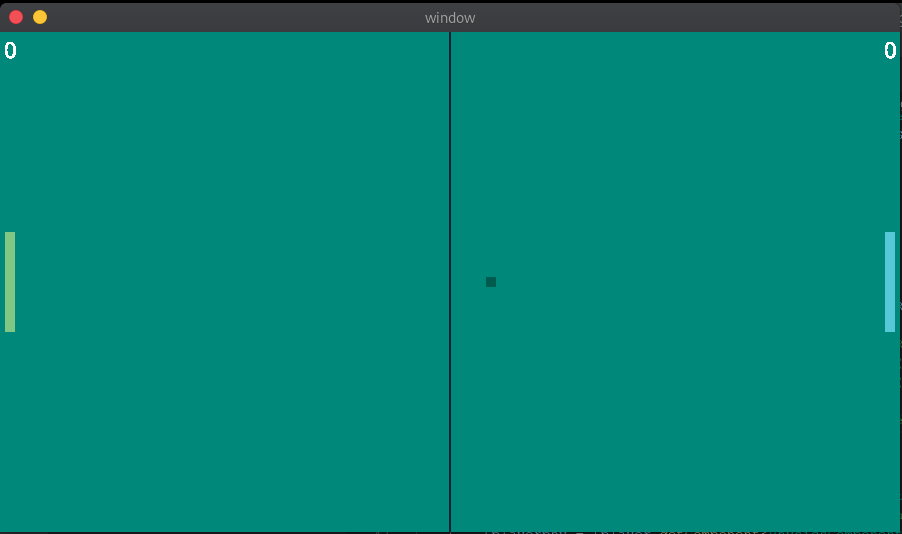
\includegraphics[width=15cm]{archivos/imagenes/pong-nuevos-colores.png}
	\caption{Imagen del Pong con nuevos colores y marcador.}
\end{figure}

Lo que hice en segunda instancia, no estaba dentro de los objetivos que nos habíamos marcado pero decidí hacer un menú, pensando que sería algo sencillo, pero me llevó más tiempo del que imaginaba. Para hacer el menú necesitaba renderizar texto, y para no alargar más el desarrollo, decidí añadir una librería que se usa para renderizar texto en formato true type llamada stb\_truetype. De esta manera, también podría usar los números del marcador como texto. Para moverte por el menú se usarán las flechas del teclado de arriba y abajo. El resultado es el siguiente:

\begin{figure}[h]
	\centering
	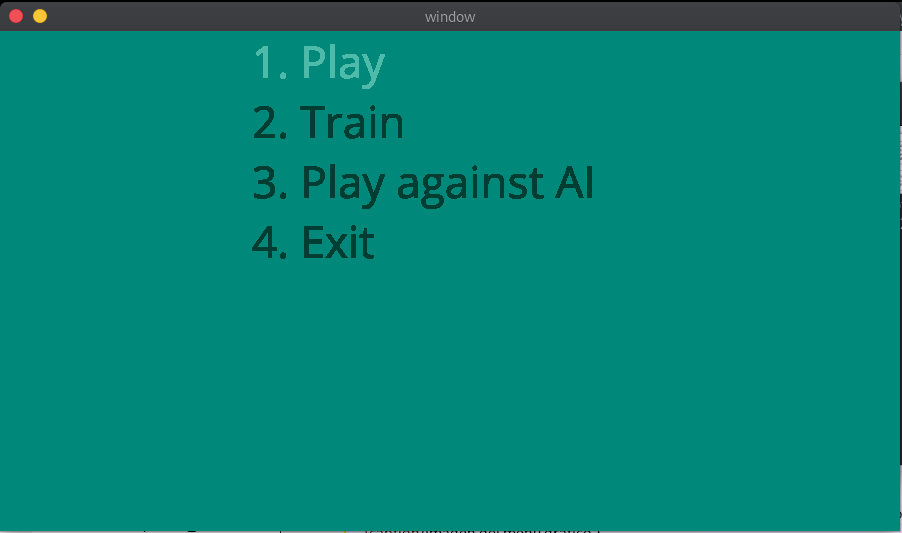
\includegraphics[width=15cm]{archivos/imagenes/menu-grafico-integrado-en-el-juego.png}
	\caption{Imagen del menú gráfico.}
\end{figure}
\todo{La imagen del menú antiguo aparece en otro sitio ¿he de arreglarlo? ¿poner una referencia? ¿cómo lo arreglo?}
Una vez acabado el menú, que además te permite seleccionar qué \gls{csv} quieres usar entre todos los que has generado jugando, añadí los minions y unas paredes, las cuales habría que romper para poder pasar tu bola al campo enemigo. Esto es posible porque las bolas traspasan las paredes que son de su mismo color.

\begin{figure}[h]
	\centering
	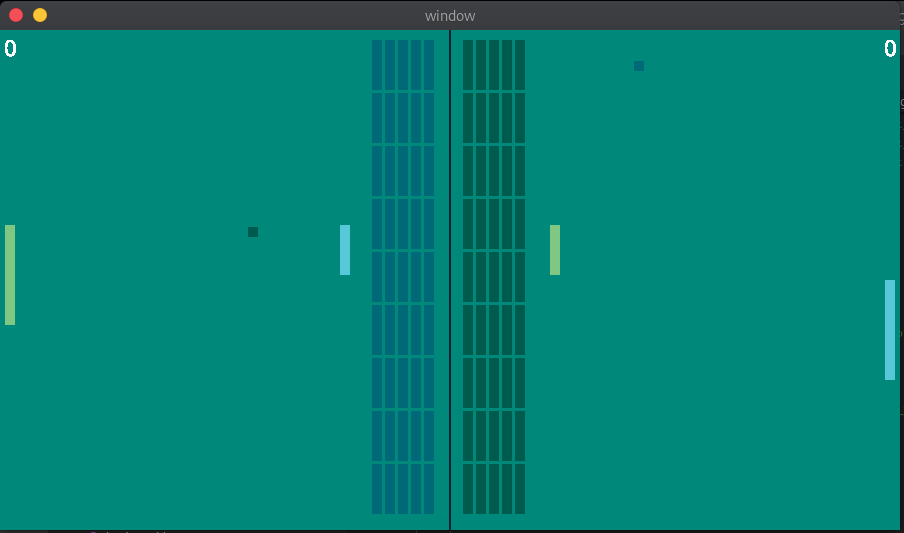
\includegraphics[width=15cm]{archivos/imagenes/pong-plus-con-minions-y-paredes.png}
	\caption{Imagen de la primera versión del Pong Plus.}
\end{figure}
\todo{La imagen del juego con muros aparece en otro sitio ¿he de arreglarlo? ¿poner una referencia? ¿cómo lo arreglo?}

\subsection{Compilación para Windows}
Lo último que hice en este periodo fue compilar el juego para Windows. Mi tutor explica en el curso de videojuegos \cite{CursoMotorC++} cómo modificar el fichero de construcción (Makefile) para compilar para Windows desde una máquina con Linux (comúnmente conocido como cross-compiling), y en la librería de TinyPTC descargable, también hay unos ficheros de código específicos para Windows, por lo que la única tarea que me quedaba por hacer era modificar las partes del código donde se incluye la versión de TinyPTC de Linux e incluir la versión de Windows, y recompilar el proyecto. 
\\
Pero cuando probé el juego en Windows, se ejecutaba correctamente, pero no respondía ante la entrada por teclado. Y es que la codificación del teclado en Windows no es la misma que la de X11, por lo que creé un fichero en el que definí los valores de la variable dependiendo de si la compilación está activada para Windows o para Linux.

\section{Sexta iteración: aprendizaje mediante backpropagation}
El \textbf{11 de febrero de 2021} tuvimos una nueva reunión, en la cual los objetivos marcados fueron:
\begin{enumerate}
	\item Continuar mejorando defectos de la memoria y desarrollando los nuevos hitos de las nuevas iteraciones.
	\item Implementar Dear ImGui en el proyecto
	\begin{itemize}
		\item Estudiar cómo se usa.
		\item Sustituir TinyPTC por OpenGL3 para poder renderizar tanto el juego como las ventanas .
		\item Diseñar menús para manejar el juego.
	\end{itemize}
	\item Programar el algoritmo de backpropagation.
	\item Poder elegir tanto los ficheros de datos de entrenamientos como los ficheros de pesos para el juego.
	\item Añadir un campo de entrenamiento para que no sea necesario que haya dos jugadores para recoger datos de entrenamiento.
	\item Añadir un algoritmo básico para cuando no exista un fichero de pesos pero que se pueda jugar contra una \gls{ia}.
\end{enumerate}

Comencé la iteración con ilusión, viendo documentación de Dear ImGui y estudiando cómo implementar la librería en mi proyecto. Pero antes de empezar a implementarlo debía acabar lo que empecé en la anterior iteración, la red neuronal. Es cierto que en la anterior iteración la red neuronal ya era capaz de resolver el problema de la XOR con un entrenamiento aleatorio, es decir, probar una asignación de pesos aleatoria para la red, y si obtenía mejores resultados que la mejor red hasta el momento, se sustituían los pesos de la red neuronal por estos nuevos.
\begin{figure}[h]
	\centering
	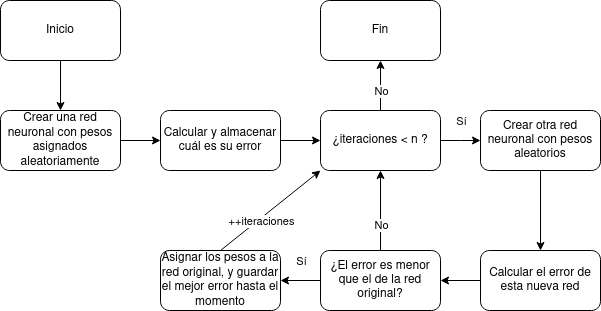
\includegraphics[width=15cm]{archivos/imagenes/Algoritmo-red-neuronal-aleatorio.png}
	\caption{Algoritmo de aprendizaje aleatorio.}
\end{figure}
Es un algoritmo que podría funcionar en algunos casos, pero requiere de un número mucho más alto de iteraciones, así que no es lo suficientemente eficiente. Por lo que me dispuse a desarrollar el algoritmo de backpropagation.

\subsection{Graves problemas durante el desarrollo}
Como ya he mencionado en el apartado de herramientas de trabajo, yo he desarrollado este proyecto con Linux, pero por motivos relacionados con la carrera, es necesario que también tenga instalado Windows en el ordenador. Después de una actualización, este último dejó de funcionar, y cuando opté por solucionar el error, se cargó la partición de Linux. Por suerte, todo el trabajo de este \gls{tfg} estaba bajo el control de Git, y en la nube de GitHub, por lo que los daños en ese sentido eran mínimos. Pero tenía que recuperar el resto de cosas.

No voy a contar cómo fue la recuperación del sistema operativo ya que no procede en esta memoria, pero esto juntado con los trabajos de las asignaturas de la universidad, me hizo perder más de una semana, por lo que esta iteración quedó prácticamente en nada.

\subsection{Explicación de backpropagation}
Después de recuperar todo el sistema operativo, continué con el desarrollo del algoritmo. El mayor problema de este es entender cómo funciona teóricamente este, ya que en código no es muy complicado de hacer una vez entiendes los índices que componen el algoritmo. Puedes ver un esquema  del funcionamiento del algoritmo en la figura \ref{Algoritmo de backpropagation}
\begin{figure}[h]
	\centering
	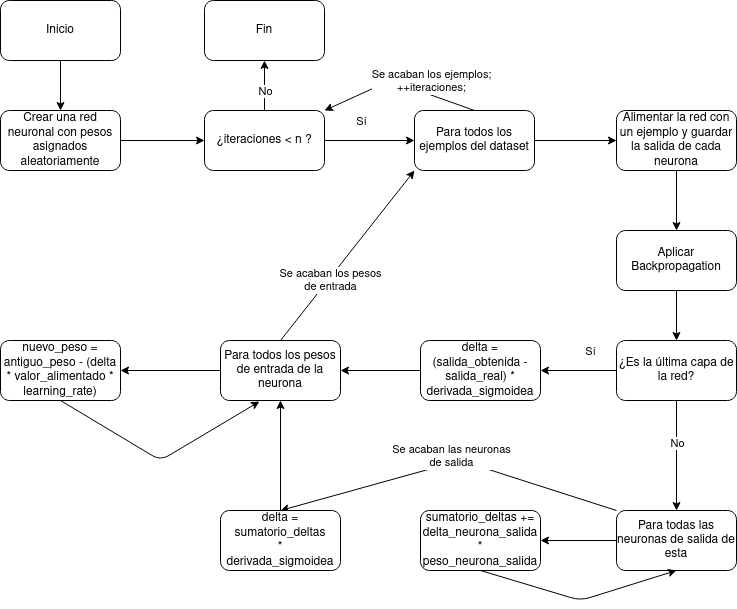
\includegraphics[width=15cm]{archivos/imagenes/Algoritmo-de-backpropagation.png}
	\caption{Algoritmo de backpropagation.}
	\label{Algoritmo de backpropagation}
\end{figure}

Y aunque parece fácil de entender viéndolo de una forma esquemática, el problema está cuando has de saber a qué índice corresponde cada fórmula en el código. Lo que haremos será escoger un ejemplo del dataset. Para cada peso de entrada (j), de cada neurona (i), de cada capa (l), vamos a aplicar la fórmula \ref{eq:descenso del gradiente} Es decir, aplica el descenso del gradiente.
\begin{subequations}
	\begin{eqnarray}
		w_{ij}^{(l)} = w_{ij}^{(l)} - \alpha*\nabla E(w_{ij}^{(l)}) \label{eq:descenso del gradiente} \\
		\nabla E(w_{ij}^{(l)}) =  \frac{\delta E(w_{ij}^{(l)})}{\delta w_{ij}^{(l)}} \label{eq:derivada parcial}
	\end{eqnarray}
\end{subequations}
El alpha que aparece, que todavía no he comentado, es el factor de aprendizaje, que hará que el descenso del gradiente sea más rápido si es más grande, pero también más errático. Y la fórmula \ref{eq:derivada parcial} representa el gradiente de la función de error, es decir, en este caso la derivada parcial respecto al peso j de la neurona i.

La función de error que estoy usando en Backpropagation es el error cuadrático, es decir, la media de la suma de los cuadrados en la fórmula \ref{Error cuadratico}. Siendo $h(x)_n$ el resultado de la red neuronal para una entrada x, $y_n$ el resultado real que debería haber obtenido, y N el número total de ejemplos. Cabe destacar que el superíndice es una ele mayúscula debido a que esto connota que la capa de la que hablamos es la última.
\begin{equation}
	\label{Error cuadratico}
	E(w_{ij}^{(L)}) = \frac{1}{N}\sum_{n=0}^N(h(x)_n - y_n)^2
\end{equation}

Pero ahora queremos calcular el gradiente del error, y para eso necesitamos saber qué es lo que vale la función \ref{eq:derivada parcial}. Para eso usaremos la regla de la cadena. Pero antes de ponernos con la fórmula, hay que entender qué significa cada símbolo. 

\begin{figure}[h]
	\centering
	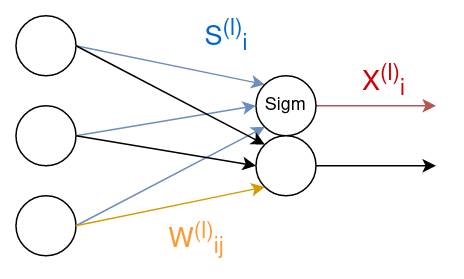
\includegraphics[width=15cm]{archivos/imagenes/Red-neuronal-simbolos.png}
	\caption{Símbolos de una red neuronal.}
	\label{fig:symb neural net}
\end{figure}

Como se puede apreciar en la figura \ref{fig:symb neural net}, la w con sus índices se refiere al peso j de una neurona i de la capa l. La S  con sus índices se refiere a la señal (sumatorio de cada entrada por cada peso) de la neurona i en la capa l. Sigm se refiere a la función de activación, la sigmoidea en este caso. Y por último x con sus índices se refiere a la salida de la neurona i (la ele minúscula indica la capa, si quisiéramos la salida de la capa anterior, que es lo que nos interesa, usaremos l-1) después de pasar por la función de activación, si fuese la capa l sería la salida de la neurona anterior.
\\
Una vez entendido cada símbolo, podemos entender la regla de la cadena que aplicamos en la fórmula \ref{Chain rule signal}. Gracias a esta regla obtenemos algo más sencillo de calcular, que es la derivada de la señal respecto al peso, mucho más sencillo de calcular como vemos en la fórmula \ref{Derivada de la señal respecto al peso}. Y a la derivada del error respecto a la señal, es a lo que llamaremos delta, que como expliqué en el marco teórico, es lo que se acumula en todas las capas, y por lo tanto lo que nos va a interesar almacenar.
\begin{subequations}
	\begin{eqnarray}
		\nabla E(w_{ij}^{(l)}) =  \frac{\delta E(w_{ij}^{(l)})}{\delta w_{ij}^{(l)}} = \frac{\delta E(w_{ij}^{(l)})}{\delta w_{ij}^{(l)}} * \frac{\delta S_{i}^{(l)}}{\delta S_{i}^{(l)}} = \frac{\delta E(w_{ij}^{(l)})}{\delta S_{i}^{(l)}} * \frac{\delta S_{i}^{(l)}}{\delta w_{ij}^{(l)}} \label{Chain rule signal} \\
		\frac{\delta S_{i}^{(l)}}{\delta w_{ij}^{(l)}} = \frac{\delta (x_{i}^{(l-1)}*w_{ij}^{(l)}) }{\delta w_{ij}^{(l)}} = x_{i}^{(l-1)} \label{Derivada de la señal respecto al peso}
	\end{eqnarray}
\end{subequations}

Pero todavía no sabemos lo que vale delta, así que volvemos a aplicar la regla de la cadena \ref{Chain rule delta}. Lo que conseguimos es obtener la derivada de la salida de la neurona después de aplicar la función de activación, respecto al sumatorio de cada entrada de la neurona por cada peso, esto es lo mismo que la derivada de la función de activación en la señal \ref{Derivada de la salida respecto a la entrada}. Y ahora ya sí que podemos obtener la derivada de la función de error respecto a la salida de la neurona \ref{Derivada de la salida de la red respecto a la salida real}.
\begin{subequations}
	\begin{eqnarray}
		\frac{\delta E(w_{ij}^{(l)})}{\delta S_{i}^{(l)}} = \frac{\delta E(w_{ij}^{(l)})}{\delta S_{i}^{(l)}} * \frac{\delta x_{i}^{(l)}}{\delta x_{i}^{(l)}} = \frac{\delta E(w_{ij}^{(l)})}{\delta x_{i}^{(l)}} * \frac{\delta x_{i}^{(l)}}{\delta S_{i}^{(l)}} \label{Chain rule delta} \\
		\frac{\delta x_{i}^{(l)}}{\delta S_{i}^{(l)}} = Sigm'(S_{i}^{(l)}) = Sigm(S_{i}^{(l)}) * (1 - Sigm(S_{i}^{(l)})) \label{Derivada de la salida respecto a la entrada} \\
		\frac{\delta E(w_{ij}^{(l)})}{\delta x_{i}^{(l)}} = \frac{\delta (h(x) - y)^2}{\delta x_{i}^{(l)}} = \frac{\delta (x_{i}^{(l)} - y_{i})^2}{\delta x_{i}^{(l)}} = 2 * (x_{i}^{(l)} - y_{i}) \label{Derivada de la salida de la red respecto a la salida real}
	\end{eqnarray}
\end{subequations}

Por lo tanto podemos concluir que el cálculo de delta, cuando estamos en la última capa L (ele mayúscula), es la fórmula \ref{Delta en la ultima capa}. Y que el gradiente para la última capa será \ref{Gradiente para las neuronas de la ultima capa}.
\begin{subequations}
	\begin{eqnarray}
		\delta_{i}^{(L)} = 2 * (x_{i}^{(L)} - y_{i}) * Sigm(S_{i}^{(L)}) * (1 - Sigm(S_{i}^{(L)})) \label{Delta en la ultima capa} \\
		\nabla E(w_{ij}^{(l)}) = \delta_{i}^{(L)}  * x_{i}^{(L-1)} \label{Gradiente para las neuronas de la ultima capa}
	\end{eqnarray}
\end{subequations}

Pero nos faltaría calcular el gradiente para las capas anteriores a la última. Como he mencionado antes, la virtud de Backpropagation es que vamos acumulando delta porque se propaga desde el final hasta el principio. Sólo tenemos que seguir la fórmula \ref{Chain rule signal}, es decir, multiplicar el nuevo delta (que todavía no conocemos y habremos de calcular) por la entrada que corresponde a ese peso. 
\\
Por lo tanto, ya sabemos cuál es la entrada de la señal  de entrada de la neurona que corresponde a ese peso \ref{Derivada de la señal respecto al peso}, y calcular el nuevo delta, usando la regla de la cadena, y teniendo en cuenta el delta de la capa posterior, sería: la derivada de la función de activación en la señal de entrada, por el delta de la neurona de salida, por el peso que conecta esa neurona con la neurona de salida \ref{Delta en el resto de capas}. 
\\
Para entender mejor de forma visual cómo se calcula el delta de la capa l, puedes ver la figura \ref{Delta en la capa l}. Se observa como, en este caso hay dos neuronas de salida que han tenido un error, acumulado en su delta, cada delta es multiplicado por el peso que le une a esa neurona porque si el peso es mayor, significa que tendrá más culpa del error, y también se aprecia que sigue apareciendo la señal de entrada de la neurona y la derivada de la sigmoidea, porque también han afectado al error y hay que tenerlo en cuenta para el nuevo delta.
\begin{subequations}
	\begin{eqnarray}
		\delta_{i}^{(l)} = Sigm'(S_{i}^{(l)}) * \sum_{j=0}^{n} \delta_{ij}^{(l+1)} * w_{ij}^{(l+1)} \label{Delta en el resto de capas} \\
		\nabla E(w_{ij}^{(l)}) = \delta_{i}^{(l)}  * x_{i}^{(l-1)} \label{Gradiente para las neuronas del resto de capas}
	\end{eqnarray}
\end{subequations}

\begin{figure}[h]
	\centering
	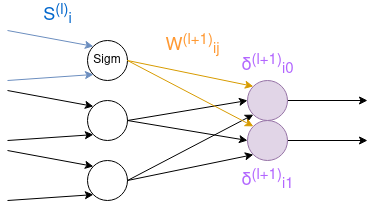
\includegraphics[width=15cm]{archivos/imagenes/Calculo-del-delta-en-la-capa-l.png}
	\caption{Cálculo de delta en la capa l $\neq$ L}
	\label{Delta en la capa l}
\end{figure}

Haremos esta operación para cada peso de cada neurona de esta capa, a ese peso le aplicaremos el gradiente como en la fórmula \ref{eq:descenso del gradiente}, y avanzaremos hacia la capa de atrás hasta que no queden más capas.

Para ver las ventajas de backpropagation de forma empírica respecto al algoritmo aleatorio, ir al apartado de resultados.....\todo{Añadir referencia al apartado resultados cuando exista}

\section{Séptima iteración: creación de menús}
El día \textbf{11 de marzo de 2021} volvimos a tener una llamada de revisión de trabajo y nuevas propuestas, pero según se desarrolló la anterior iteración, mi tutor y yo acordamos que para esta acabaría lo ya acordado, prestando especial atención en el desarrollo de la memoria, ya que era lo que más trabajo requería en la situación en la que estaba, y conociendo que ya quedaba poco tiempo para la entrega del \gls{tfg}.

\subsection{Dear ImGui}
Por lo tanto, comencé a implementar Dear ImGui en el proyecto. El primer paso era sustituir TinyPTC por OpenGL3, así que eso hice: fui al sistema de Render, que se encarga de abrir la ventana y dibujar sobre ella, y cambié todo el código necesario en este punto. Ahora la ventana la abriría con OpenGL3 y cada frame dibujado por software mediante el sistema de render se pasaría a OpenGL3 también, de esta manera Dear ImGui solo tendrá que dibujar las ventanas encima de mi interfaz.
\\
El siguiente paso fue aprender a dibujar una ventana dentro del juego, y así fue, algo bastante sencillo porque aparece en el código de ejemplo que ellos tienen en el proyecto.
\missingfigure{Añadir imagen de una ventana sobre el juego}
Pero como los menús de los juego no suelen ser en una ventana, decidí hacerlo en pantalla completa. No es el mejor diseño, pero ya servía para poder manejarse  dentro del juego.
\missingfigure{Añadir imagen del menu del juego}
Ahora ya, teniendo las herramientas que nos da Dear ImGui, me dispuse a desarrollar un menú en el cuál el jugador, pueda decidir cómo entrenar a su \gls{ia}, y además que pueda ver de manera gráfica cómo va aprendiendo y cuáles son las consecuencias de cambiar los parámetros de entrenamiento de la \gls{ia}.
\missingfigure{Añadir  imagen del menu de entrenamiento}

\subsection{Campo de entrenamiento}
\todo{Explicar el campo de entrenamiento}

\section{Octava iteración: perfilando el proyecto}
El \textbf{13 de abril de 2021} ya solo quedaba un mes para la confirmación de la entrega del proyecto en el C3, por lo que ya tendríamos que tener todo acabado para esta fecha, o a punto de acabar para confirmar. Los objetivos para esta iteración, por lo tanto, fueron los siguientes:
\begin{enumerate}
	\item Añadir capturas a la memoria, puesto que eran escasas y eran necesarias para entenderla.
	\item Añadir apartado de resultados a la memoria, con tablas, imágenes, y demás representaciones.
	\item Arreglar el método de entrenamiento de la \gls{ia}.
	\item Añadir un algoritmo básico para cuando no exista un fichero de pesos pero que se pueda jugar contra una \gls{ia}.
\end{enumerate}

\section{Novena iteración: ...}
El día \textbf{6 de mayo de 2021} fue la última iteración antes de decidir si entregaríamos el \gls{tfg} ..........